\documentclass[25pt, a0paper, portrait, margin=10mm, innermargin=15mm,
blockverticalspace=15mm, colspace=15mm, subcolspace=8mm]{tikzposter}
\usepackage{natbib}
%\usepackage{pgfplots}
\usepackage[default]{lato}
\usepackage{concrete}
\usepackage[utf8]{inputenc}
\usepackage{graphics}
%\pgfplotsset{/pgf/number format/use comma,compat=1.7}

\definecolor{blau1}{RGB}{0,105,170}
\definecolor{blau2}{RGB}{80,170,200}
\definecolor{rot}{RGB}{198,24,38}
\definecolor{sand}{RGB}{244,241,234}
\definecolor{braun}{RGB}{89,13,8}
\definecolor{green}{RGB}{77,175,74}
\definecolor{red}{RGB}{228,26,28}
\definecolor{purple}{RGB}{152,78,163}
\definecolor{blue}{RGB}{55,126,184}
\tikzstyle{nonterm}=[rounded corners,draw=blue!50,fill=blue!20,thick,font=\sffamily]
\tikzstyle{vroot}=[rounded corners,draw=gray!50,fill=gray!20,thick,font=\sffamily]
\tikzstyle{nontermedge}=[line width=1.5pt,draw=black!50]
\tikzstyle{vrootedge}=[line width=1.5pt,draw=gray!20]
\tikzstyle{termcell}=[matrix,inner sep=1pt,row sep=0pt,matrix anchor=north west]
\tikzstyle{terminal}=[rectangle,font=\small]
\tikzstyle{edgelabel}=[rectangle,draw=gray!50,fill=gray!20,font=\sffamily\tiny]

\usecolorstyle[colorTwo=braun,colorThree=sand,colorOne=rot]{Australia}

\titlegraphic{
\includegraphics[height=10cm]{logo-University-of-Heidelberg}}
\title{Rule-based Corefence Resolution with BART}
\institute{Institute for Computational Linguistics, Univ. Heidelberg}
\author{Julian Baumann, Xenia Kühling, Sebastian Ruder}
\makeatletter
\makeatother

\begin{document}\maketitle
\begin{columns} \column{0.55}
\block{Creating the document}{The document...} \note[targetoffsetx=.15\textwidth,targetoffsety=4.5cm,innersep=.4cm,angle=245]{Optional...}
\block{The title matter}{The title...}
\block{Blocks}{Blocks are...} \note[targetoffsetx=-1cm, targetoffsety=-10cm,rotate=5,angle=270,radius=8cm,width=.35\textwidth,innersep=.4cm]{You
can...}

\column{0.45} \block{Columns}{By default,...}
\begin{subcolumns} \subcolumn{.4} \block{Subcolumns}{If you...} \subcolumn{.5} \block{}{An example...} \end{subcolumns}
\block[titlewidthscale=.8,bodywidthscale=.9,titleoffsety=7.5mm,bodyoffsety=7mm]{Changing the Poster’s Appearance}{If the default...}
\block{image}
{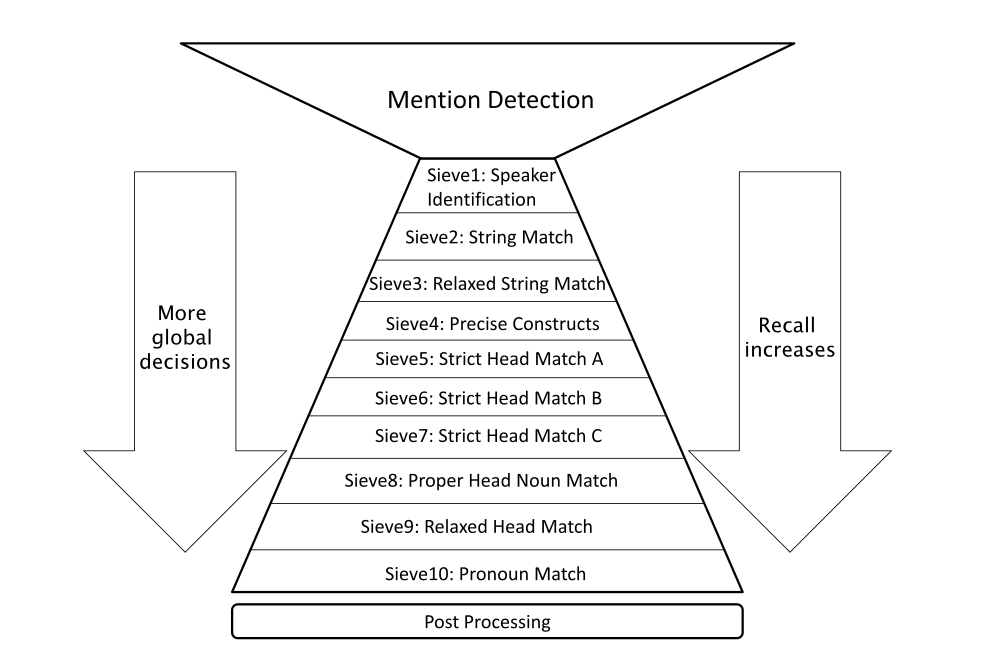
\includegraphics{stanford}}
\end{columns}


\end{document}
